\item A thin rod of mass $M$ and length $a$ is free to rotate in horizontal plane about a fixed vertical axis passing through point O. A thin circular disc of mass $M$ and radius $a/4$ is pivoted on this rod with its center at a distance $a/4$ from the free end so that it can rotate freely about its vertical axis, as shown in the figure. Assume that both the rod and the disc have uniform density and they remain horizontal during the motion. An outside stationary observer finds the rod rotating with an angular velocity $\Omega$ and the disc rotating about its vertical axis with angular velocity $4\Omega$. The total angular momentum of the system about the point O is $(Ma^{2}\Omega/48)n$. The value of $n$ is \underline{\hspace{2.5 cm}}. 
    
    \begin{center}
        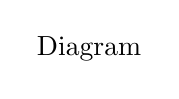
\begin{tikzpicture}
            \node {Diagram};
        \end{tikzpicture}
    \end{center}

    \begin{solution}
        \begin{center}
            \begin{tikzpicture}
                \tzcoor*(0, 0)(O){$O$}[bl]
                \tzcoor*(30:2)(C){$C$}[br]
                \tzcoor*(60:3)(P){$P$}[ar]
                \tzline[->](O)(C){$\vec{r}_{CO}$}[mb]
                \tzline[->](C)(P){$\vec{r}_{PC}$}[mr]
                \tzline[->](O)(P){$\vec{r}_{PO}$}[ml]
            \end{tikzpicture}
        \end{center}
    
        \begin{align*}
            \vec{L}_P &= \vec{r}_P \times \vec{p} \\
                      &= (\vec{r}_C + \vec{r}_{\text{particle}}) \times (m \cdot \vec{v}) \\
                      &= \vec{r}_C \times (m \cdot \vec{v}) + \vec{r}_{\text{particle}} \times (m \cdot \vec{v}) \\
                      &= m \cdot \vec{r}_{\text{particle}} \times \vec{\omega}_1 \\
                      &= m \cdot (\vec{r}_C + \vec{r}_{\text{particle}}) \times \vec{\omega}_1 \\
                      &= m \cdot \vec{r}_C \times \vec{\omega}_1 + m \cdot \vec{r}_{\text{particle}} \times \vec{\omega}_1 \\
                      &= m \cdot \vec{r}_P \times \vec{\omega}_1 \\
                      &= I_P \cdot \vec{\omega}_1 + m \cdot \vec{r}_P \times \vec{\omega}_2
            \end{align*}

         
            \setlength{\jot}{10pt}
                    \begin{align*}   
                        \intertext{Given:}
                        \vec{L} &= \vec{r} \times \vec{p} &&\quad \text{(Angular momentum definition)} \\
                        \intertext{For the particle rotating around point C:}
                        \vec{L}_C &= \vec{r}_C \times \vec{p} &&\quad \text{(Angular momentum with respect to point C)} \\
                                  &= I_C \cdot \vec{\omega}_1 &&\quad \text{(Using \( \vec{p} = I_C \cdot \vec{\omega}_1 \))} \\
                        \intertext{Now, considering the rotation of point C around point P:}
                        \vec{L}_P &= \vec{r}_P \times \vec{p} &&\quad \text{(Angular momentum with respect to point P)} \\
                                  &= (\vec{r}_C + \vec{r}_{\text{particle}}) \times (m \cdot \vec{v}) &&\quad \text{(Expanding)} \\
                                  &= \vec{r}_C \times (m \cdot \vec{v}) + \vec{r}_{\text{particle}} \times (m \cdot \vec{v}) &&\quad \text{(Using distributive property)} \\
                                  &= m \cdot \vec{r}_{\text{particle}} \times \vec{\omega}_1 &&\quad \text{(Substituting \( \vec{v} = \vec{\omega}_1 \times \vec{r}_C \))} \\
                                  &= m \cdot (\vec{r}_P - \vec{r}_C) \times \vec{\omega}_1 &&\quad \text{(Using \( \vec{r}_{\text{particle}} = \vec{r}_P - \vec{r}_C \))} \\
                                  &= m \cdot \vec{r}_P \times \vec{\omega}_1 - m \cdot \vec{r}_C \times \vec{\omega}_1 &&\quad \text{(Expanding)} \\
                                  &= m \cdot \vec{r}_P \times \vec{\omega}_1 &&\quad \text{(Since \( \vec{r}_C \) is constant)} \\
                                  &= m \cdot \vec{r}_P \times \vec{\omega}_2 &&\quad \text{(Using \( \vec{\omega}_1 = \vec{\omega}_2 \times \vec{r}_C \))} \\
                                  &= I_P \cdot \vec{\omega}_1 + m \cdot \vec{r}_P \times \vec{\omega}_2 &&\quad \text{(Substituting \( I_P = I_C + m \cdot r^2 \))}
                    \end{align*}
                        
    


\begin{align*}
\intertext{The position vector of point P:}
\vec{r}_P &= \vec{r}_C + \vec{r}_{PC} \\
\intertext{The velocity of point P:}
\vec{v}_P &= \vec{v}_C + \vec{v}_{PC} \\
\intertext{Relating the velocity $\vec{v}_{PC}$ to the angular velocity $\vec{\omega}_1$:}
\vec{v}_{PC} &= \vec{\omega}_1 \times \vec{r}_{PC} \\
\intertext{The velocity $\vec{v}_C$ in terms of angular velocity $\vec{\omega}_2$:}
\vec{v}_C &= \vec{\omega}_2 \times \vec{r}_C \\
\intertext{Angular momentum of the particle with respect to point P:}
\vec{L}_P &= \vec{r}_P \times \vec{p} \\
&= (\vec{r}_C + \vec{r}_{\text{particle}}) \times (m \cdot \vec{v}) \\
&= \vec{r}_C \times (m \cdot \vec{v}) + \vec{r}_{\text{particle}} \times (m \cdot \vec{v}) \\
\end{align*}
\begin{align*}
    \textbf{1. Position vectors:} \\
    \intertext{Define the position vector of the particle with respect to point C as $\mathbf{r}$}
    \intertext{Define the position vector of point C with respect to point P as $\mathbf{R}$}
    \intertext{Therefore, the position vector of the particle with respect to point P is $\mathbf{r'} = \mathbf{R} + \mathbf{r}$} \\
    \textbf{2. Velocity vectors:} \\
    \intertext{The velocity of the particle with respect to point C is $\mathbf{v_1} = \boldsymbol{\omega_1} \times \mathbf{r}$ (cross product of angular velocity and position vector)} 
    \intertext{The velocity of point C with respect to point P is $\mathbf{v_2} = \boldsymbol{\omega_2} \times \mathbf{R}$}
    \intertext{Using the relative velocity concept, the velocity of the particle with respect to point P is $\mathbf{v} = \mathbf{v_1} + \mathbf{v_2}$} \\
    \textbf{3. Linear momentum:} \\
    \intertext{The linear momentum of the particle is $\mathbf{p} = m \cdot \mathbf{v}$} \\
    \textbf{4. Angular momentum about point P:} \\
    \intertext{Using the definition $\mathbf{L} = \mathbf{r'} \times \mathbf{p}$, we get:}\\
    &\mathbf{L} = \mathbf{r'} \times (m \cdot \mathbf{v}) \\
    &\mathbf{L} = (\mathbf{R} + \mathbf{r}) \times (m \cdot (\mathbf{v_1} + \mathbf{v_2})) \\
    \intertext{Expanding the cross product:}\\
    &\mathbf{L} = \mathbf{R} \times (m \cdot \mathbf{v_1}) + \mathbf{R} \times (m \cdot \mathbf{v_2}) + \mathbf{r} \times (m \cdot \mathbf{v_1}) + \mathbf{r} \times (m \cdot \mathbf{v_2}) \\ 
    \textbf{5. Analyzing the terms:} \\
    \intertext{The terms represent different contributions to the angular momentum:} \\
    \intertext{- $\mathbf{R} \times (m \cdot \mathbf{v_1})$: Angular momentum due to particle's rotation around C, as seen from P.}
    \intertext{- $\mathbf{R} \times (m \cdot \mathbf{v_2})$: Angular momentum due to the motion of point C around P.}
    \intertext{- $\mathbf{r} \times (m \cdot \mathbf{v_1})$: Angular momentum of the particle due to its own rotation around C.}
    \intertext{- $\mathbf{r} \times (m \cdot \mathbf{v_2})$: This term is zero (r and v2 are parallel)}\\
    \textbf{6. Final expression:} \\
    \intertext{Therefore, the angular momentum in vector form is:} \\
    &\mathbf{L} = m \cdot (\mathbf{R} \times \mathbf{v_1} + \mathbf{R} \times \mathbf{v_2} + \mathbf{r} \times \mathbf{v_1}) \\
    \intertext{Substituting v1 and v2 with their respective cross products:} \\
    \mathbf{L} = m \cdot (\mathbf{R} \times (\boldsymbol{\omega_1} \times \mathbf{r}) + \mathbf{R} \times (\boldsymbol{\omega_2} \times \mathbf{R}) + \mathbf{r} \times (\boldsymbol{\omega_1} \times \mathbf{r}))
    \end{align*}
\end{solution}

